\documentclass[a4paper,ngerman,landscape]{scrartcl}

\usepackage[utf8]{inputenc}

\usepackage[ngerman]{babel}
\usepackage{hyperref}

\usepackage{graphicx}
\usepackage{tikz}
\usetikzlibrary{calc}

\usepackage[protrusion=true,expansion=true]{microtype}

\usepackage{libertine}
\usepackage{tabto}

\setlength\parskip{\medskipamount}
\setlength\parindent{0pt}

\usepackage{geometry}
\geometry{tmargin=0.1cm,bmargin=1.0cm,lmargin=1.5cm,rmargin=1.5cm}

\pagestyle{empty}

\begin{document}

\begin{center}
  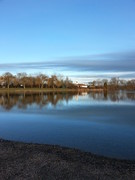
\includegraphics[height=0.15\textwidth]{eisbaden-4}
  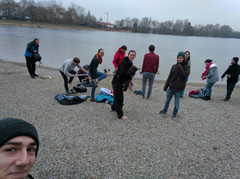
\includegraphics[height=0.15\textwidth]{eisbaden-3}
  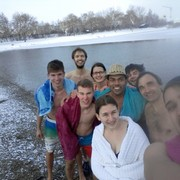
\includegraphics[height=0.15\textwidth]{eisbaden-1}
  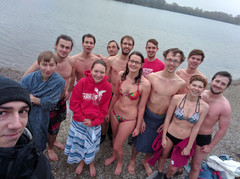
\includegraphics[height=0.15\textwidth]{eisbaden-2}
  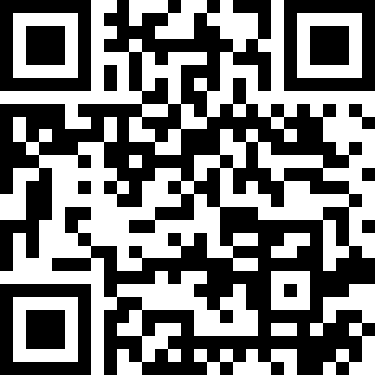
\includegraphics[height=0.15\textwidth]{eisbaden-qrcode}

  \Huge
  \scalebox{3.8}{\textbf{Mathe-Eisbaden}}

  \large
  \begin{minipage}{0.92\textwidth}
    \renewcommand{\baselinestretch}{1.3}

    \setlength\parskip{\medskipamount}
    \vspace{0.3em}
    Eisbaden macht Spaß, tut gut und ist nicht so krass, wie man es sich vorstellt.
    Wir haben das schon öfter gemacht. Das nächste Mal wird es das große
    offizielle Institutseisbaden. Alle Interessierten sind herzlich eingeladen.
    Wir treffen uns am Dienstag möglichst pünktlich nach 11:30 Uhr bei der
    Schranke zwischen Mathe- und Info-Gebäude, um dann gemeinsam zum Ilsesee in
    Königsbrunn zu fahren. Um 12:15 Uhr sind wir wieder an der Uni.
    Wer mit möchte, muss sich nur auf \textsf{http:/$\!$/bit.ly/2jYnmEt} eintragen, damit
    wir die Anzahl Autos planen können.
    \vspace{0.3em}
  \end{minipage}

  \huge
  \scalebox{1.5}{Dienstag, 24. Januar 2017, 11:30--12:15 Uhr}

  % http://www.taz.de/picture/233361/948/eisbaden-koepper.jpg
  \tikz[remember picture,overlay] \node[opacity=1.0,inner sep=0pt] at (current
  page.south){\hspace*{-3cm}\vbox{\vspace*{-6.4cm}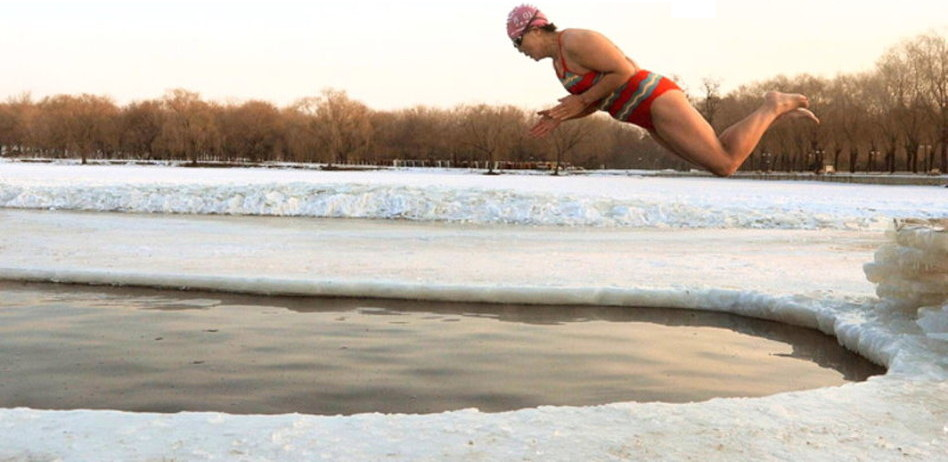
\includegraphics[width=\paperwidth]{eisbaden-sprung}}};
\end{center}

\end{document}
